\documentclass[tikz,14pt,fleqn]{article}

% Math
\usepackage[fleqn]{amsmath}
\usepackage{amssymb}
\usepackage{dsfont}
\usepackage{float}

% Insert dummy text
\usepackage{lipsum}  
% Allows to use caption*
\usepackage{caption}
% Scalabale subfigures
\usepackage{subcaption} 
% Code syntax highlighting
\usepackage{minted}
% Hyperlinks
\usepackage{hyperref}
% Customize page layout
\usepackage{geometry}
\geometry{a4paper, margin=1in}
% Page headers and footers
\usepackage{fancyhdr}
\pagestyle{fancy}
\fancyhf{}
\setlength{\parindent}{0pt}
\setlength{\parskip}{0.5\baselineskip}%

% includegraphics
\usepackage{graphicx}




\newcommand{\bmat}[1]{
   \ensuremath{
   \begin{bmatrix}
       #1
   \end{bmatrix}
}}




\usepackage[utf8]{inputenc}


%%%%%%%%%%%%%%%%%%%%%%%%%%%%
%% VARIABLES
\newcommand\namesurname{Albert Cerfeda}
\newcommand\assignment{Assignment 4 - Color and Multi-scale Representations}

\newcommand\subject{Image \& Video Processing}
\newcommand\documentdate{29 May 2023}

% Title content
%%%%%%%%%%%%%%%%%%%%%%%%%%%%
\rhead{\assignment}
\lhead{\namesurname}
%%%%%%%%%%%%%%%%%%%%%%%%%%%%

\rfoot{Page \thepage}


\begin{document}

\begin{titlepage}
   \begin{center}
       \vspace*{0.2cm}

       \textbf{\Large{\subject}}

       \vspace{0.5cm}
        \textbf{\assignment}\\[5mm]
        
            
       \vspace{0.4cm}

        \namesurname
        \begin{figure}[H]
            \centering
        \end{figure}
       \tableofcontents

       \vspace*{\fill}
     
        
\includegraphics[width=0.4\textwidth]{fig/logo.png}
       
        \documentdate \\
        Università della Svizzera italiana\\
        Faculty of Informatics\\
        Switzerland\\

   \end{center}
\end{titlepage}

\section{Color Palette Extraction from Images [7 points]}
\subsection{Linear RGB and sRGB Color Palettes}

\begin{figure}[h!]
    \vspace*{-0.2cm}
    \inputminted[firstline=90, frame=lines, framesep=2mm, fontsize=\small ]{matlab}{../src/ex1.m}
    \vspace*{-0.5cm}
    \caption{Matlab code performing color quantization}
\end{figure}



\begin{figure}[h!]
    \centering
    \begin{subfigure}[]{\linewidth}
        \centering
        
\includegraphics[width=0.13\linewidth]{fig/out/1.1.rgb_palette_1.png}
        
\includegraphics[width=0.13\linewidth]{fig/out/1.1.rgb_palette_2.png}
        
\includegraphics[width=0.13\linewidth]{fig/out/1.1.rgb_palette_3.png}
        
\includegraphics[width=0.13\linewidth]{fig/out/1.1.rgb_palette_4.png}
        
\includegraphics[width=0.13\linewidth]{fig/out/1.1.rgb_palette_5.png}
        
\includegraphics[width=0.13\linewidth]{fig/out/1.1.rgb_palette_6.png}
        
\includegraphics[width=0.13\linewidth]{fig/out/1.1.rgb_palette_7.png}\\
        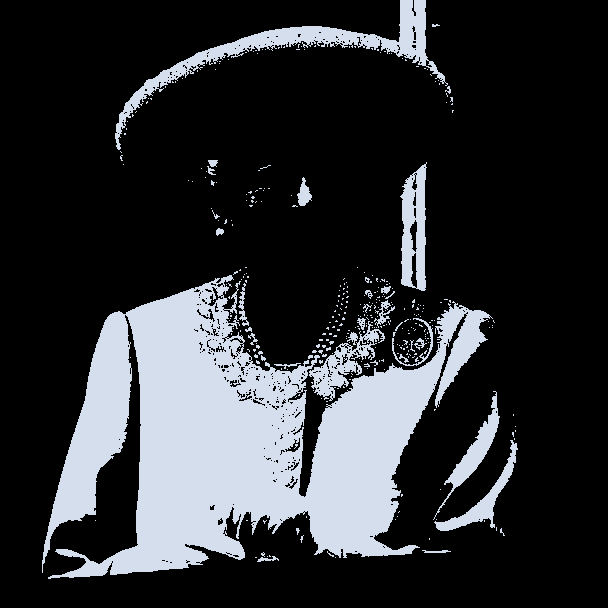
\includegraphics[width=0.13\linewidth]{fig/out/1.1.rgb_layer_1.png}
        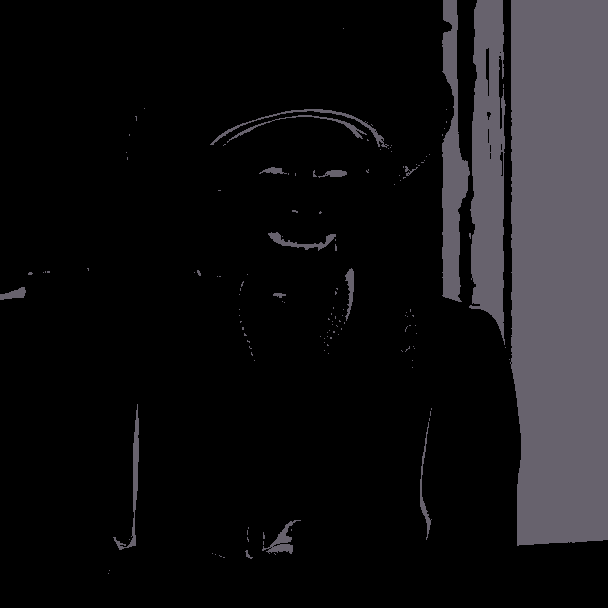
\includegraphics[width=0.13\linewidth]{fig/out/1.1.rgb_layer_2.png}
        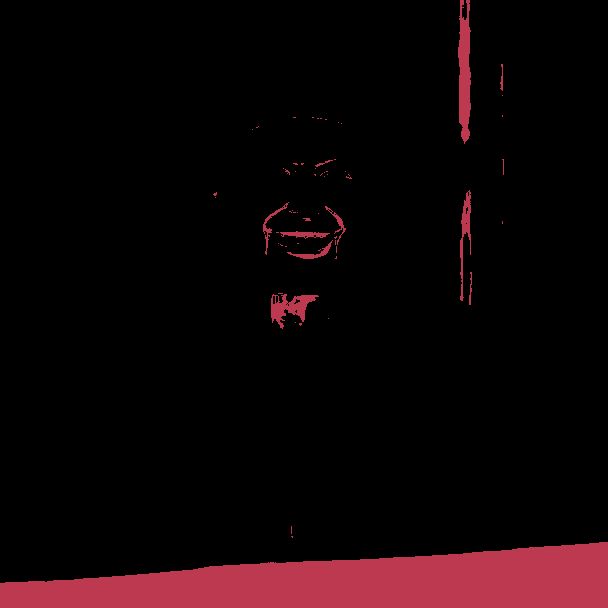
\includegraphics[width=0.13\linewidth]{fig/out/1.1.rgb_layer_3.png}
        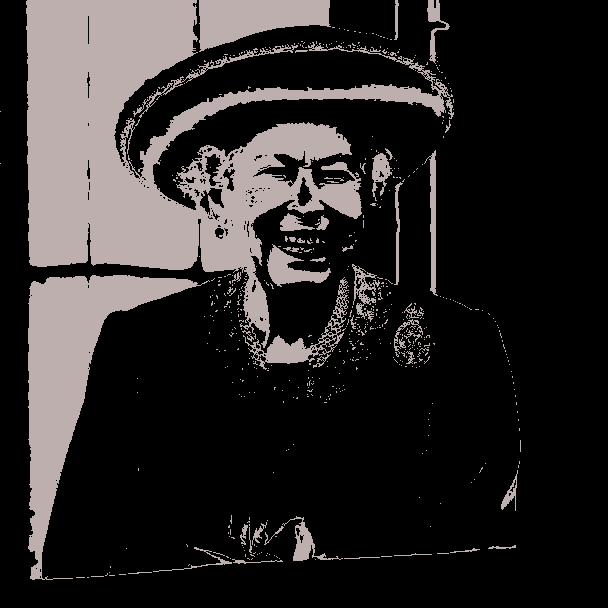
\includegraphics[width=0.13\linewidth]{fig/out/1.1.rgb_layer_4.png}
        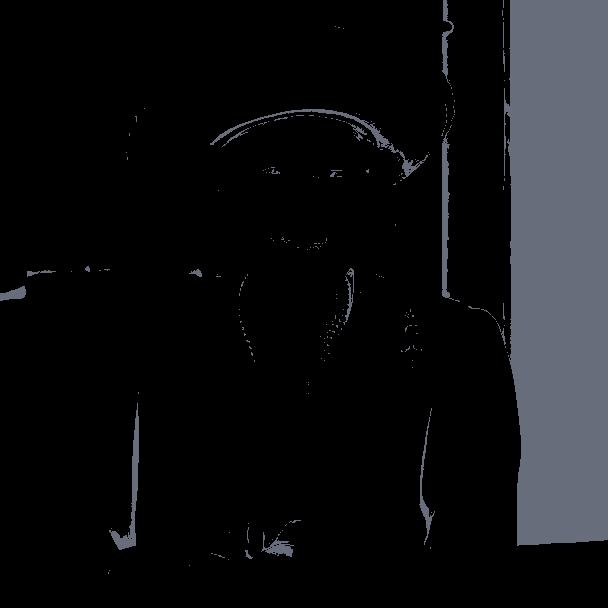
\includegraphics[width=0.13\linewidth]{fig/out/1.1.rgb_layer_5.png}
        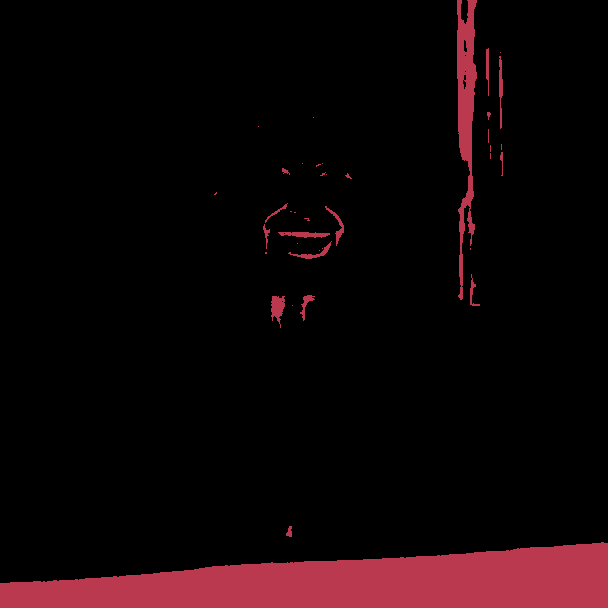
\includegraphics[width=0.13\linewidth]{fig/out/1.1.rgb_layer_6.png}
        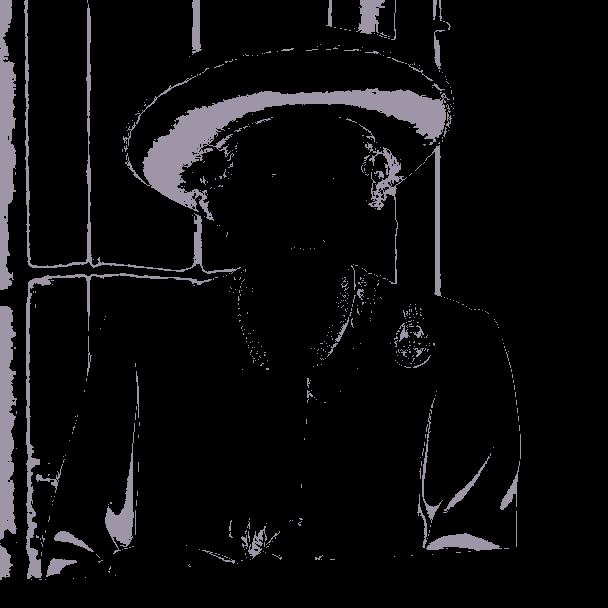
\includegraphics[width=0.13\linewidth]{fig/out/1.1.rgb_layer_7.png}
        \caption{RGB Palette and Layers}
        \label{fig:1.1.rgb_palette_layers}
    \end{subfigure}
    \begin{subfigure}[]{\linewidth}
        \centering
        
\includegraphics[width=0.13\linewidth]{fig/out/1.1.xyz_palette_1.png}
        
\includegraphics[width=0.13\linewidth]{fig/out/1.1.xyz_palette_2.png}
        
\includegraphics[width=0.13\linewidth]{fig/out/1.1.xyz_palette_3.png}
        
\includegraphics[width=0.13\linewidth]{fig/out/1.1.xyz_palette_4.png}
        
\includegraphics[width=0.13\linewidth]{fig/out/1.1.xyz_palette_5.png}
        
\includegraphics[width=0.13\linewidth]{fig/out/1.1.xyz_palette_6.png}
        
\includegraphics[width=0.13\linewidth]{fig/out/1.1.xyz_palette_7.png}\\
        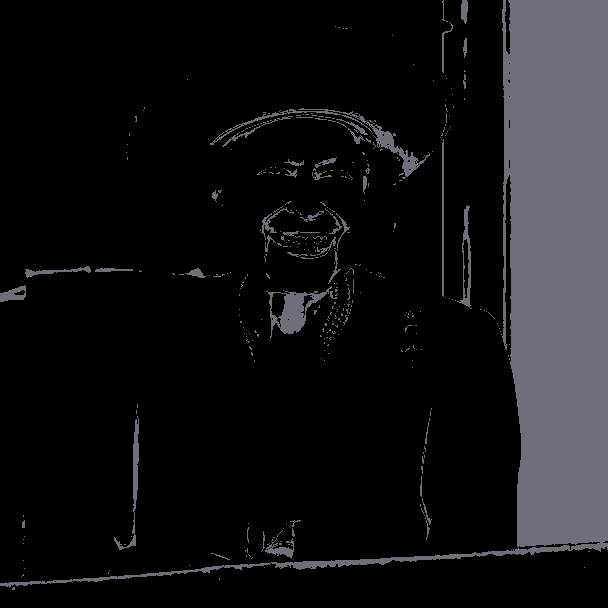
\includegraphics[width=0.13\linewidth]{fig/out/1.1.xyz_layer_1.png}
        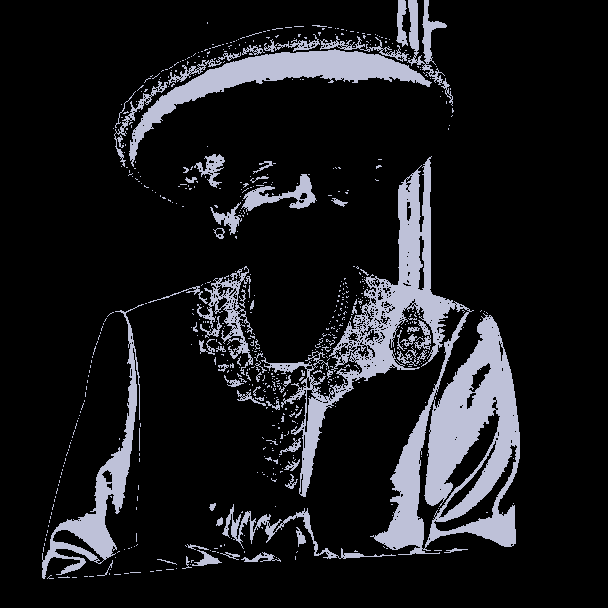
\includegraphics[width=0.13\linewidth]{fig/out/1.1.xyz_layer_2.png}
        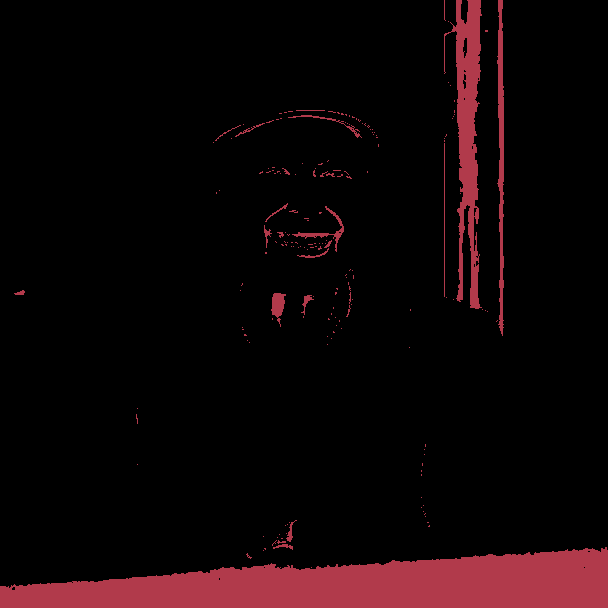
\includegraphics[width=0.13\linewidth]{fig/out/1.1.xyz_layer_3.png}
        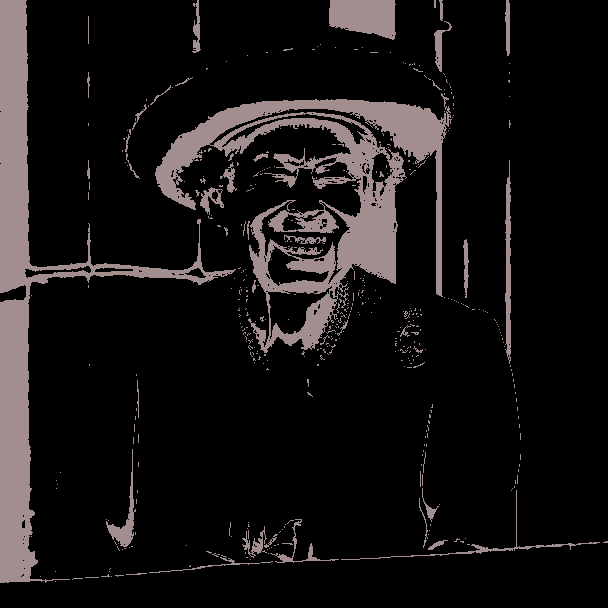
\includegraphics[width=0.13\linewidth]{fig/out/1.1.xyz_layer_4.png}
        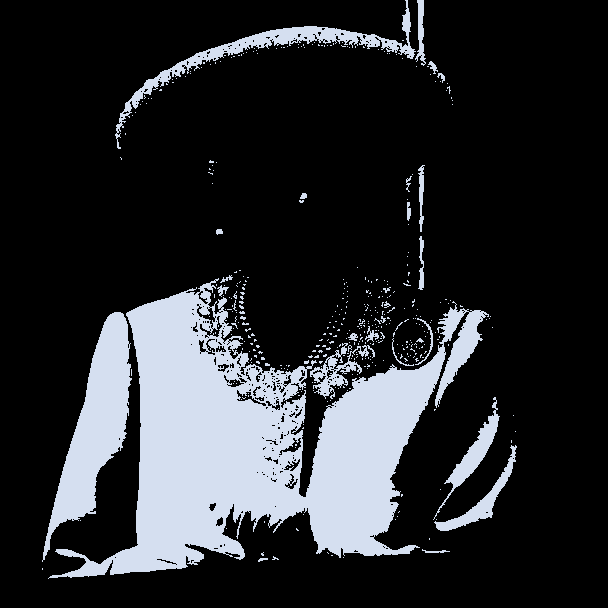
\includegraphics[width=0.13\linewidth]{fig/out/1.1.xyz_layer_5.png}
        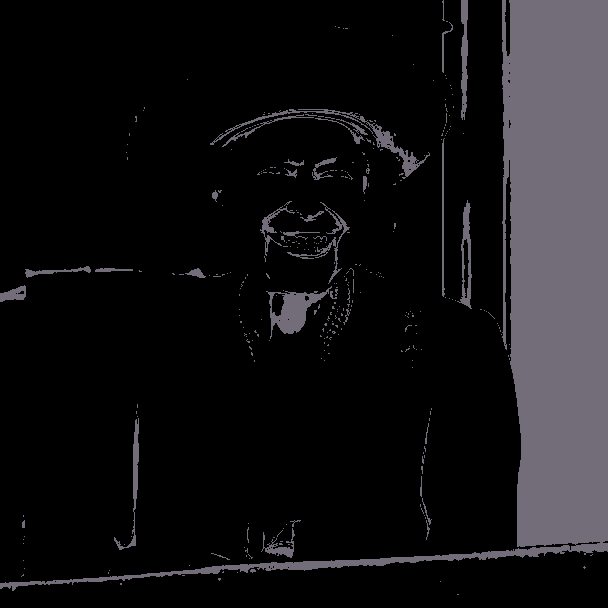
\includegraphics[width=0.13\linewidth]{fig/out/1.1.xyz_layer_6.png}
        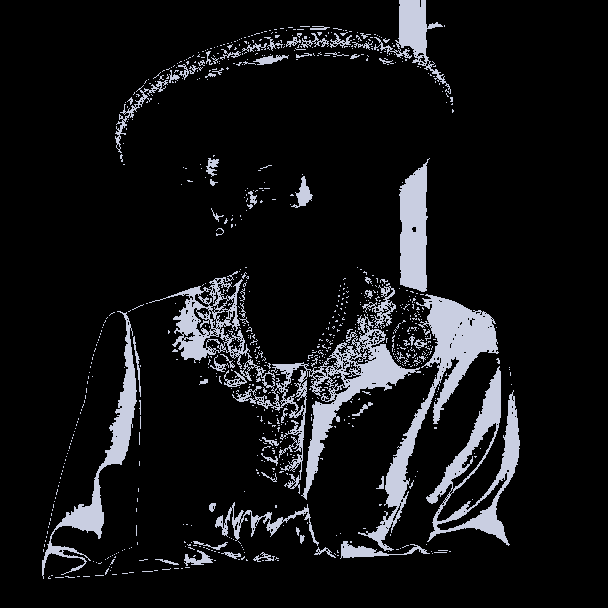
\includegraphics[width=0.13\linewidth]{fig/out/1.1.xyz_layer_7.png}
        \caption{sRGB Palette and Layers}
        \label{fig:1.1.srgb_palette_layers}
    \end{subfigure}
    \begin{subfigure}[]{0.25\linewidth}
        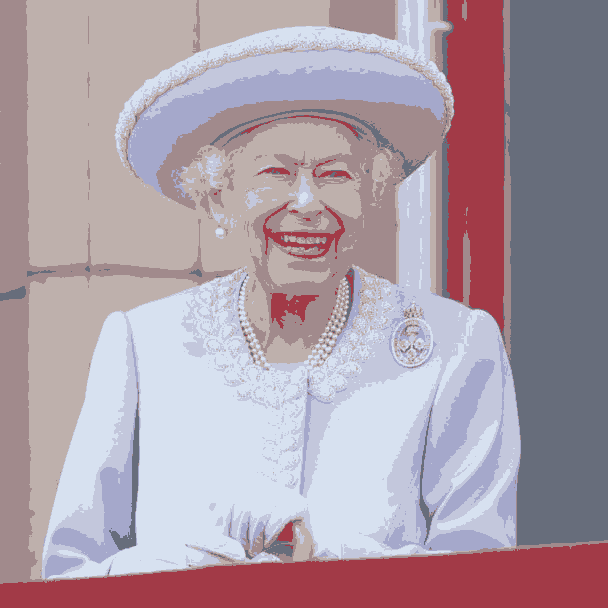
\includegraphics[width=\linewidth]{fig/out/1.1.rgb_clustered.png}
        \caption{RGB Clustered image}
        \label{fig:1.1.rgb_clustered}
    \end{subfigure}
    \begin{subfigure}[]{0.25\linewidth}
        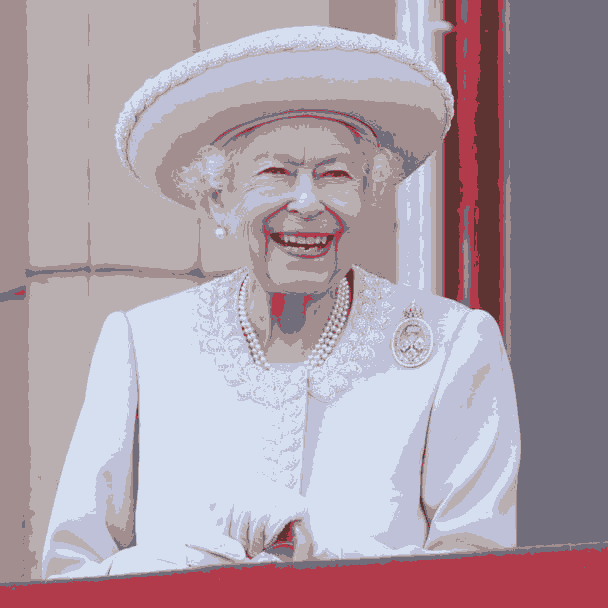
\includegraphics[width=\linewidth]{fig/out/1.1.xyz_clustered.png}
        \caption{sRGB Clustered image}
        \label{fig:1.1.srgb_clustered}
    \end{subfigure}
    \caption{Color palette extraction using the RGB and sRGB color spaces.}
\end{figure}


\subsection{CIELab Color Palette}


\section{Color Quantization and lookup tables (LUTs) [3 points]}
\begin{figure}
    \begin{subfigure}[]{0.245\linewidth}
        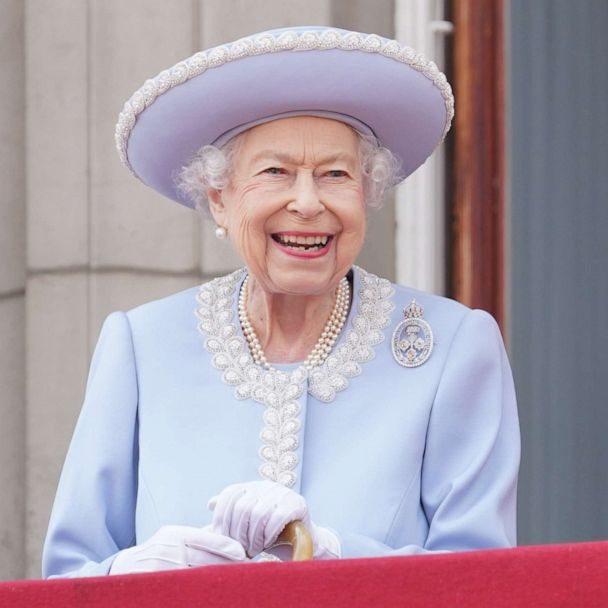
\includegraphics[width=\linewidth]{fig/out/2.img.png}
        \caption{Original image}
        \label{fig:2.img}
    \end{subfigure}
    \begin{subfigure}[]{0.245\linewidth}
        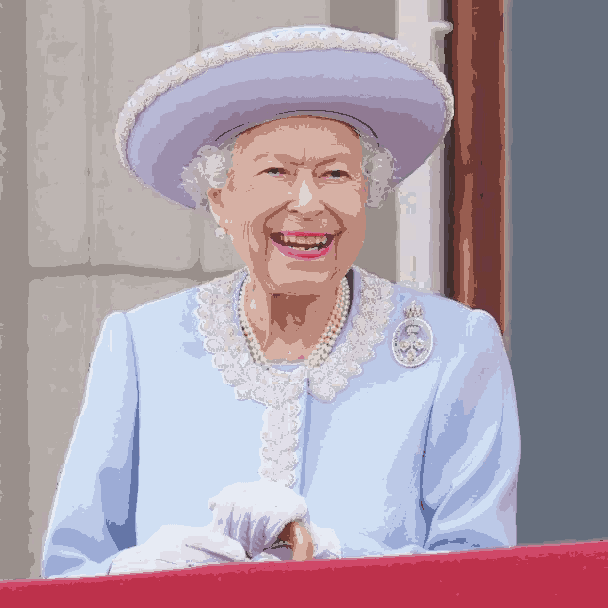
\includegraphics[width=\linewidth]{fig/out/2.hsv.png}
        \caption{HSV color space}
        \label{fig:2.hsv}
    \end{subfigure}
    \begin{subfigure}[]{0.245\linewidth}
        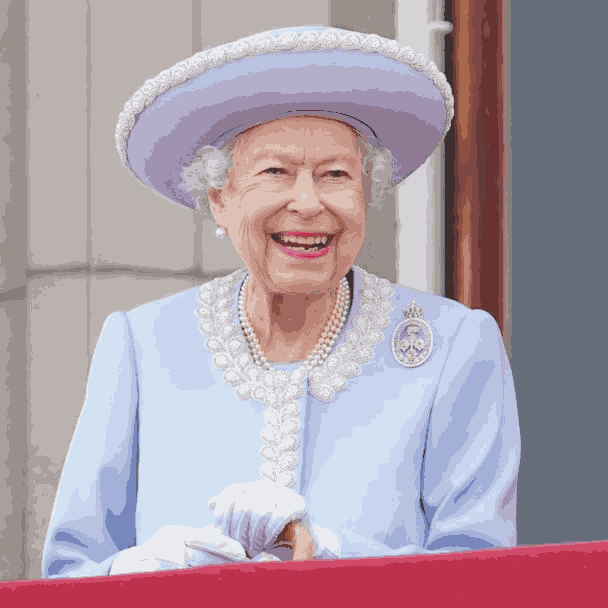
\includegraphics[width=\linewidth]{fig/out/2.lab.png}
        \caption{CIELab color space}
        \label{fig:2.lab}
    \end{subfigure}
    \begin{subfigure}[]{0.245\linewidth}
        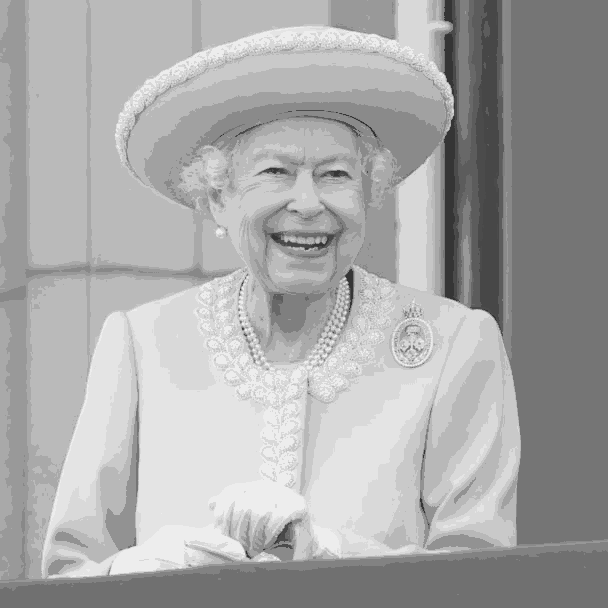
\includegraphics[width=\linewidth]{fig/out/2.gray.png}
        \caption{Grayscale-mapped}
        \label{fig:2.gray}
    \end{subfigure}
    \caption{Quantized images with 32 clusters (colors) in different color spaces}
    \label{fig:2}
\end{figure}



\section{Gaussian and Laplacian Pyramids [4 points]}

\begin{figure}[h!]
    \vspace*{-0.2cm}
    \inputminted[firstline=57, frame=lines, framesep=2mm, fontsize=\small ]{matlab}{../src/ex3.m}
    \vspace*{-0.5cm}
    \caption{Matlab functions computing the Gaussian and Laplacian pyramids and reconstructing the original image.}
\end{figure}

\begin{figure}[h!]
    \centering
    \begin{subfigure}[]{.7\linewidth}
        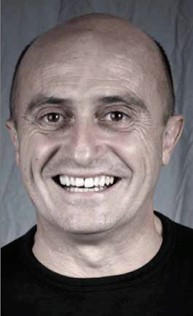
\includegraphics[height=0.3\linewidth]{fig/out/3.happy_gaussian_pyramid_1.png}
        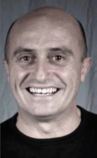
\includegraphics[height=0.3\linewidth]{fig/out/3.happy_gaussian_pyramid_2.png}
        
\includegraphics[height=0.3\linewidth]{fig/out/3.happy_gaussian_pyramid_3.png}
        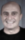
\includegraphics[height=0.3\linewidth]{fig/out/3.happy_gaussian_pyramid_4.png}
        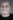
\includegraphics[height=0.3\linewidth]{fig/out/3.happy_gaussian_pyramid_5.png}
        \caption{Gaussian Pyramid layers}
    \end{subfigure}
    \begin{subfigure}[]{.7\linewidth}
        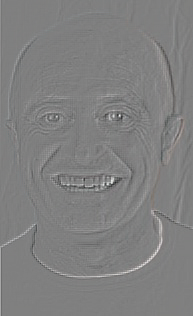
\includegraphics[height=0.3\linewidth]{fig/out/3.happy_laplacian_pyramid_1.png}
        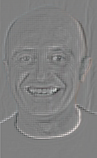
\includegraphics[height=0.3\linewidth]{fig/out/3.happy_laplacian_pyramid_2.png}
        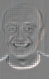
\includegraphics[height=0.3\linewidth]{fig/out/3.happy_laplacian_pyramid_3.png}
        
\includegraphics[height=0.3\linewidth]{fig/out/3.happy_laplacian_pyramid_4.png}
        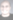
\includegraphics[height=0.3\linewidth]{fig/out/3.happy_laplacian_pyramid_5.png}     
        \caption{Laplacian Pyramid layers (brightness artifically increased)}
    \end{subfigure}
    \caption{Image pyramid decomposition of \texttt{happy.jpg}}
\end{figure}




\section{Hybrid Images [3 points]}

\begin{figure}[h!]
    \centering
    \begin{subfigure}[]{\linewidth}
        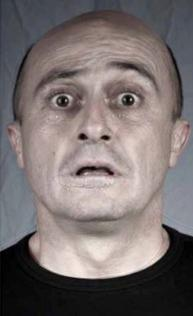
\includegraphics[width=.09\linewidth]{fig/out/4.hybrid_sigma(0.5).jpg}
        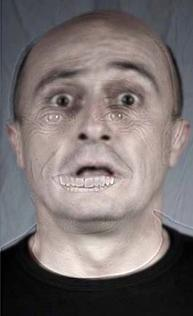
\includegraphics[width=.09\linewidth]{fig/out/4.hybrid_sigma(1.0).jpg}
        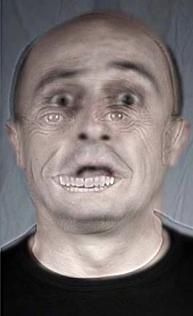
\includegraphics[width=.09\linewidth]{fig/out/4.hybrid_sigma(1.5).jpg}
        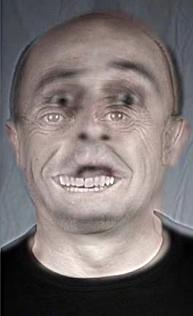
\includegraphics[width=.09\linewidth]{fig/out/4.hybrid_sigma(2.0).jpg}
        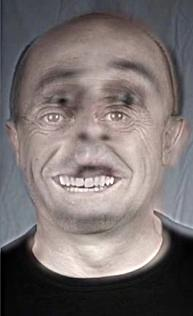
\includegraphics[width=.09\linewidth]{fig/out/4.hybrid_sigma(2.5).jpg}
        \includegraphics[width=.09\linewidth]{fig/out/4.hybrid_sigma(3.0).jpg}
        \includegraphics[width=.09\linewidth]{fig/out/4.hybrid_sigma(3.5).jpg}
        \includegraphics[width=.09\linewidth]{fig/out/4.hybrid_sigma(4.0).jpg}
        \includegraphics[width=.09\linewidth]{fig/out/4.hybrid_sigma(4.5).jpg}
        \includegraphics[width=.09\linewidth]{fig/out/4.hybrid_sigma(5.0).jpg}
    \end{subfigure}
    \caption{Hybrid images with different $\sigma$ values. Lower-Higher $\sigma$ from left to right.}
    \label{fig:4.hybrids}
\end{figure}

\begin{figure}[h!]
    \centering
    \begin{subfigure}[]{.8\linewidth}
        \begin{subfigure}[]{.25\linewidth}
            \includegraphics[width=\linewidth]{fig/out/4.hybrid_sigma(2.5).jpg}
        \end{subfigure}
        \begin{subfigure}[]{.2\linewidth}
            \includegraphics[width=\linewidth]{fig/out/4.hybrid_sigma(2.5).jpg}
        \end{subfigure}
        \begin{subfigure}[]{.16\linewidth}
            \includegraphics[width=\linewidth]{fig/out/4.hybrid_sigma(2.5).jpg}
        \end{subfigure}
        \begin{subfigure}[]{.128\linewidth}
            \includegraphics[width=\linewidth]{fig/out/4.hybrid_sigma(2.5).jpg}
        \end{subfigure}
        \begin{subfigure}[]{.1024\linewidth}
            \includegraphics[width=\linewidth]{fig/out/4.hybrid_sigma(2.5).jpg}
        \end{subfigure}
        \begin{subfigure}[]{.08192\linewidth}
            \includegraphics[width=\linewidth]{fig/out/4.hybrid_sigma(2.5).jpg}
        \end{subfigure}
    \end{subfigure}
    \caption{Showcase of frequency band sensitivity of the human visual system related to the image size.}
    \label{fig:4.showcase}
\end{figure}
\section{Theory: Hybrid Images [3 points]}


\section{Bonus: Create your own Instagram Filter! [10 points]}


\begin{figure}[h!]
    \vspace*{-0.2cm}
    \inputminted[firstline=15, frame=lines, framesep=2mm, fontsize=\small ]{matlab}{../src/ex6.m}
    \vspace*{-0.5cm}
    \caption{Matlab function applying the \textit{Borderlands 2} filter.}
\end{figure}

\begin{figure}[h!]
    % \vspace*{-0.8cm}
\end{figure}

\begin{figure}[h!]
    \centering
    \begin{subfigure}[t]{.245\linewidth}
        \includegraphics[width=\linewidth]{fig/out/6.img.jpg}
        \caption{1. Original image}
        \label{fig:6.img}
    \end{subfigure}
    \begin{subfigure}[t]{.245\linewidth}
        \includegraphics[width=\linewidth]{fig/out/6.img_clustered.jpg}
        \caption{2. Quantized image}
        \label{fig:6.img_clustered}
    \end{subfigure}
    \begin{subfigure}[t]{.245\linewidth}
        \includegraphics[width=\linewidth]{fig/out/6.img_clustered_edges.jpg}
        \caption{3. Edges of quantized image}
        \label{fig:6.img_clustered_edges}
    \end{subfigure}
    \begin{subfigure}[t]{.245\linewidth}
        \includegraphics[width=\linewidth]{fig/out/6.im_stylized.jpg}
        \caption{4. Masked and saturated final image}
        \label{fig:6.im_stylized}
    \end{subfigure}
\end{figure}


\end{document}